
\chapter{Surface treatments} % Main chapter title

\label{Chapter2.5} % Change X to a consecutive number; for referencing this chapter else where, use \ref{ChapterX}



%-----------------------------------
%	SECTION 3
%-----------------------------------
\section{Oxidation}
Room temperature oxidization is a common way of nanodiamond purification. With different oxidizing temperature, different types of impurities can be removed from the surface of the nanodiamond, ranging from water and physisorbed organic impurities, amourphous carbon, and graphitic shells and ultimate the $sp^{3}$ phase of diamond[T.Gaebel,2010]. After the oxidation, carbonyl and carboxyl groups are formed on the surface[Petrakov,2012]. Several paper have mentioned temperature choices for oxidation aiming at impurity removal. During the master's thesis period, 2 different oxidation has been examined.

\subsection[first Oxidation]{first Oxidation}
As reported, it is possible to achieve the removal of $sp^{2}$ carbon without any oxidation on $sp^{3}$ carbon via aerobic oxidation with temperature between 375$^{o}C$ and 450$^{o}C$. With temperature lower than 500$^{o}C$, the size reducing rate of nanodiamond is lower than 1nm/h. As our first treatment, we carried out a two step oxidation on sample 1508 and 1509, to achieve the complete removal of graphitic defect on the surface and light oxidation on the surface. Sample 1508 was spin coated with nanodiamond batch2, sample 1509 was spin coated with nanodiamond batch1.

The aerobatic oxidation is carried out in a tube furnace and it is done with the help of Markus Mohr. The tube furnace consists of a glass tube connected to the room atmosphere and heating coils around the glass tube. The glass tube can be slide in or out of the heating coils. We put our sample inside a ceramic sample holder and put the holder into the glass tube carefully, after the temperature has been raised to 460$^{o}C$, the glass tube was slide into the heating coils. The sample was oxidized at 460$^{o}C$ for 90min,then 480$^{o}C$ for 40min. After the Oxidation, the glass tube was slide out and the sample stayed inside the tube until it reached room temperature.

Before the oxidation, the samples was first mapped with a room temperature setup that resembles fig. 2.4, but without vaccum pump and cryostat. To make a map of SiV$^{-}$ containing points of interest, it was first taken, a scan with green laser while the fluorescence was recorded by APD, which offers us a confocal microscopy image of the sample, then the photoluminescnce spectra of the bright spots were taken, coordinates of those ones with a sharp peak at 737nm saved as points of interests for the reference of further examine.

\begin{figure}[h]
\centering
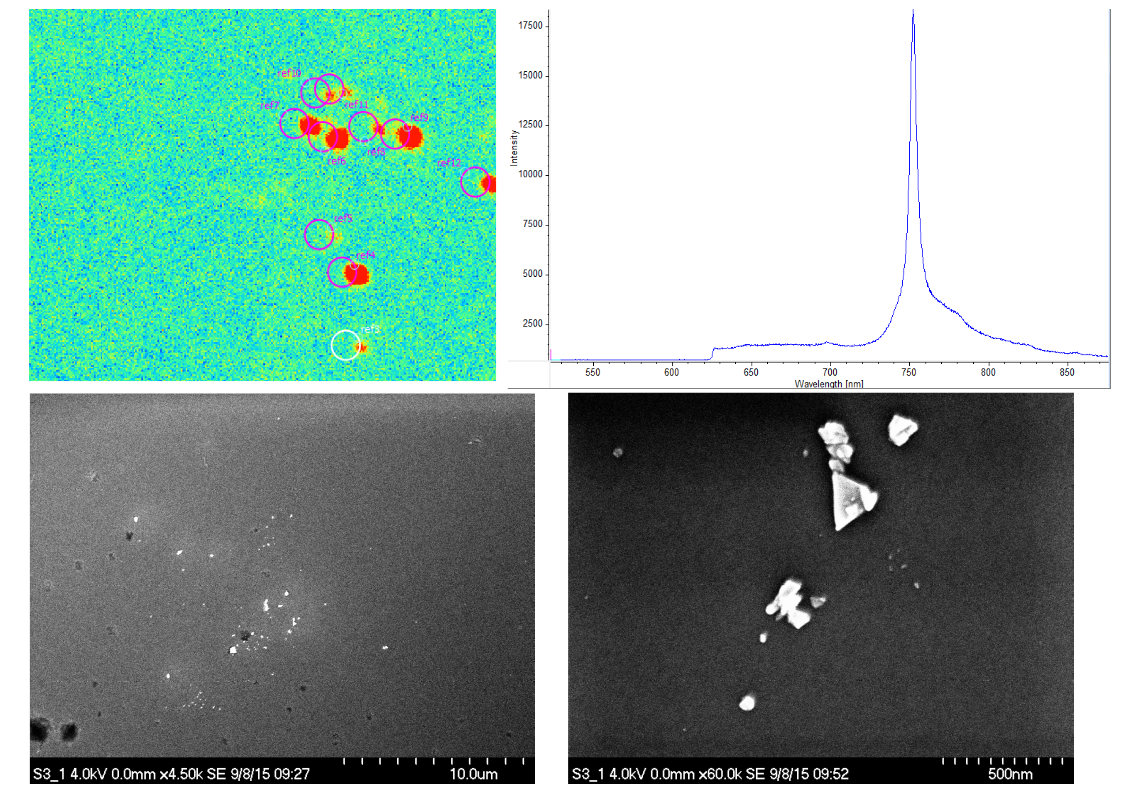
\includegraphics[width=1\linewidth]{Figures/pic/RTPL}
\caption{A)confocal image of a region of interest. The bright spots with circle markers are points of interest. B)Room temperature spectrum of a poi recorded by spectrometer. C)the roi in SEM. D)ref10 and 11 in SEM.}
\label{fig:2015-09-07-ow-capture-20150907151210-744-1}
\end{figure}

Once the map was acquired, we bring the samples to the electron microscope center and observed the regions of interest with SEM. SEM showed that, sample1508 contains more big single crystals that are larger than 300nm and clusters, while sample 1509 contains more single crystal with under 200nm sizes. This proved that the size selection via centrifuging has worked.
 
The samples was then attached to an cold finger and the placed inside the cryostat, after UHV condition has been achieved, the helium transfer was started, which would brought the temperature of the sample down to 4.8K. Most of the mapped pois are refound. Excitation with 532nm green laser double checked the existence of SiV. After the confirmation, it has been tried to carry out a resonance excitation with Titan Sapphire laser, when observing a few points of interest next to marker 5A in sample1509, it was noticed that while scanning the red laser across the line with the help of very low amount of 532nm for repopulation, a spectral diffusion of 6GHz in 15Min has been observed. To exclude the possibility of instrumental error, PLE has been operated on the bulk diamond sample with also SiV inside, where no spectral diffusio has been observed(Fig. 3.2). It has also been noticed that the increase of green laser power can cause more severe spectral drift/jump. In a case when the power green laser is brought up for a better refocus, the line has shifted totally out of the range of the spectra scan, and didn't recover in 10min. This observation brought difficulty in the measurement of orbital T1, since we always need to initialize the obital states with green laser, and this spectral diffusion that is related to the application of green laser can result in the fail of hitting the resonant wavelength, since it is technically difficult to refind the line and adjust the wavelength of the resonance laser coordinately. 

\begin{figure}[h]
\centering
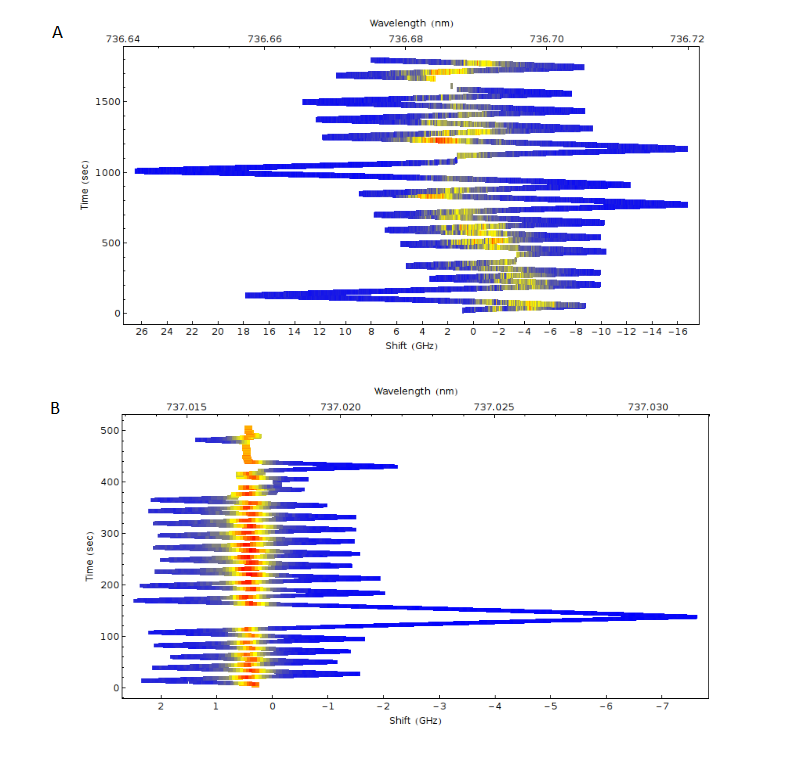
\includegraphics[width=0.7\linewidth]{Figures/pic/PLE}
\caption{PLE scan over time on A) ref5A$\textunderscore$014 from sample1509 and B) a SiV$^{-}$ site from bulk diamond sample 33b. No significant spectral diffusion been found in bulk diamond sample, which exclude the possibility of instrumental error.}
\label{fig:ple}
\end{figure}

After the obeservation above, we want to study more about this spectral diffusion behaviour that is associated with the green laser. We noticed that the sudden jump/diffusion when more green power is applied can be larger than 20GHz, maybe it is easier to track the movement of the lines with the high resolution grating of spectrometer than with PLE.

To observe the diffusion with a spectrometer, we introduced time-resolved photoluminescen spectrum, which has been described in last chapter. Due to the technical problem, our motorized sample stage can not move ideally in the vertical direction anymore, which has limited our region of observation. This time we refound the ROI around the marker 4C. And recorded the time-resolved spectrum. A session is set to be 60 spectra taken consecutively. At first, to feel the long term diffusing better, 3 sessions, with a refocus after each, are undergone for each points of interests. Since line diffusion in PLE gets wider when raising the green laser power, we excite the sample with 500uW power in front of the objective lens to obtain more diffusion. As a result, line diffusion up to 1nm has been observed.Sequentially we decrease the input power to examine the power dependency of spectral

\paragraph{post-oxidation characterisation}

After the oxidation, we noticed that the surface of the sample turned very dirty. I is yet not clear, what the contaminations are, are they intrinsic or are they extrinsic. A possible explanation is that, the contamination comes from the glass tube of tube furnace, that the residues of previous treatments has attached to the inner surface of the tube and evaporized again, depositing on the surface of our sample. Further improvement of oxidation operation has been done in our second oxidation test, and will be mentioned in the next part of the thesis.

1. Optical microscopy check
The first thing we found after the oxidation is that, the surface of our sample turned very dirty. We are yet not certain about what the contaminations are, are they intrinsic or are they external. A possible deduction is that, the contamination comes from the glass tube of tube furnace, that the residues of previous treatments has attached to the inner surface of the tube and evaporized again, depositing on the surface of our sample. Further improvement of oxidation operation has been done in our second oxidation test, and will be mentioned in the next part of the thesis.


2. Refound poi with RT setup
Huge amount of bright spots can be seen in the confocal image when we excite the sample with 532nm green laser. There's no Silicon vacancy like spectra found in these bright spots. We refind our points of interests next to the marker 4C. The photoluminescence spectra shows much higher intensity than before the oxidation.


3. Cold spectra and PLE 
After the confirmation of points of interests, the sample was transfered into the flow cryostat and the helium flow brought the temperature down to 4.8K.

At 4.8K we recorded the time-resolved photoluminescence spectra of different incident beam power with an excitation wavelength of 532nm. 

After the first oxidation, we learned that due to the inner strain of photonic fibre, the incident beam can not preserve a static polarisation. To stable the polarisation, we used a polarising beam spliter with a LC noise eater behind it. This would fix the polarisation at vertical direction.

The spectra appeared to be different from before oxidation, the most obvious change is the increase of the luminescence intensity, another observation is the broaden of the peaks and the decrease of peak number per spectra. The broadening can be caused by the misalighment of the spectrometer or the poor contact between the sample and indium, or between the sample mount and the cold finger. 

We recorded the time-resolved PL spectra, in data proceeding of post characterisation, we noticed some slow diffusion, that is not obvious when only one session is taken. So we decided to take 2 session per poi and 90s per session.

Due to the external sourced contamination, a few poi has gained a very noisy background, which leads to none ideal result.






\FloatBarrier
\begin{figure}[h]
\centering
\includegraphics[width=0.7\linewidth]{Figures/pic/WP_20160921_20_41_09_Pro_LI}
\caption{}
\label{fig:wp20160921204109proli}
\end{figure}
\FloatBarrier

\subsection[Second Oxidation]{second Oxidation}

\paragraph{method} As is mentioned before, the optical properties of SiV in bulk diamond is extraordinary. Most importantly, the spectrodiffusion that we have observed in nanodiamonds has never been seen in bulk diamonds. In the first oxidation, it seems the removal of graphitic impurity didn't help with the stablization of emiision lines. In this second oxidation, we decided to used a higher temperature to acquire a surface with groups that imitates the bulk diamond.As reported by [paper], after 2 hours of aerobatic oxidation at $575^{o}C$, ... here insert a sentence of the surface groups of nanodiamonds. To increase the chance of finding smaller nanodiamonds that would fit into a cavity and decrease the chance of getting clusters of nanodiamonds, this time we chose to use nanodiamond of the first batch. These nanodiamond are spin coated on the substrate following the method II(the index, can be change).
\FloatBarrier
\begin{figure}[h]
\centering
\includegraphics[width=0.7\linewidth]{Figures/pic/WP_20160921_20_42_21_Pro_LI}
\caption{}
\label{fig:wp20160921204221proli}
\end{figure}
\FloatBarrier
Taking the experiences of last oxidation into consideration. This time we introduces flowing inert gas (helium) to flush away the potential contaminations during the cooling process. This can also prevent the result to be affected by the humidity of the air.
We found out the extinction rate of polarising beam spliter is not ideal, so this time we used a Clan Thompson polarisation filter instead.

\paragraph{Before Oxidation}
1.Optical microscopy observation
\FloatBarrier
\begin{figure}[h]
\centering
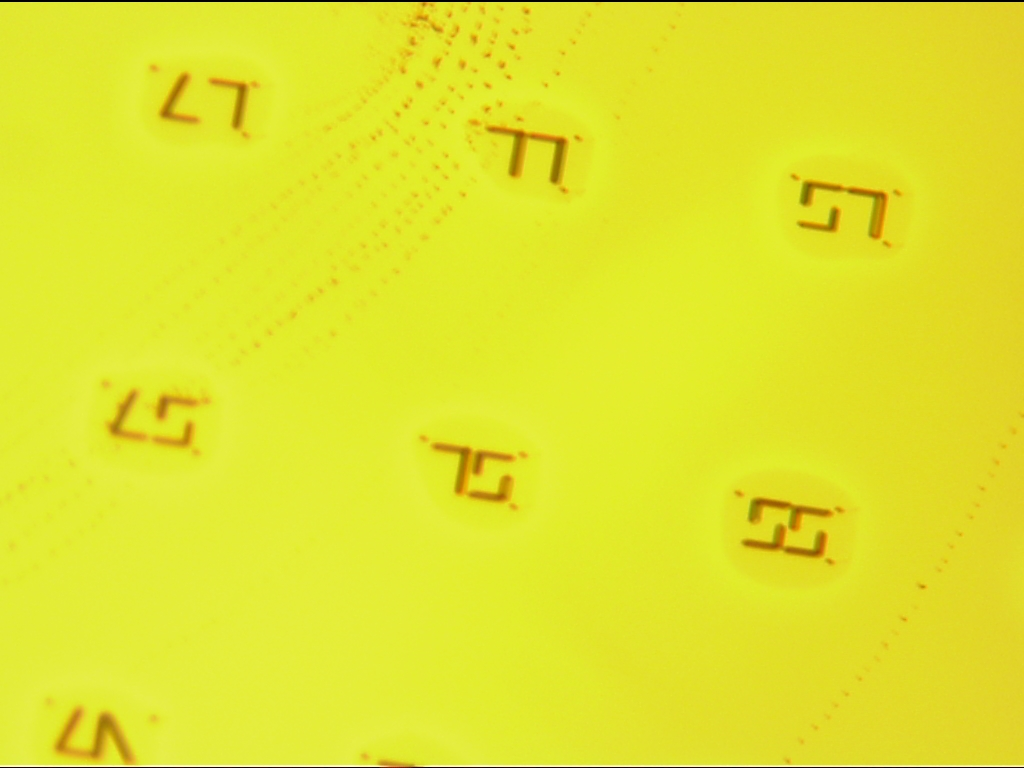
\includegraphics[width=0.7\linewidth]{Figures/pic/20150907_sample214_spincoated_5}
\caption{}
\label{fig:20150907sample214spincoated5}
\end{figure}
\FloatBarrier  
THIS IS NOT THE RIGHT FIGURE NEED CHECK THE SERVER
We observed the sample after the spin coating with optical microscopy, the surface appeared to be relatively clean, little amount of contamination has been observed, but is acceptable.

2.Mapping of $SiV^{-}$ with room temperature setup.
\FloatBarrier
\begin{figure}[h]
\centering
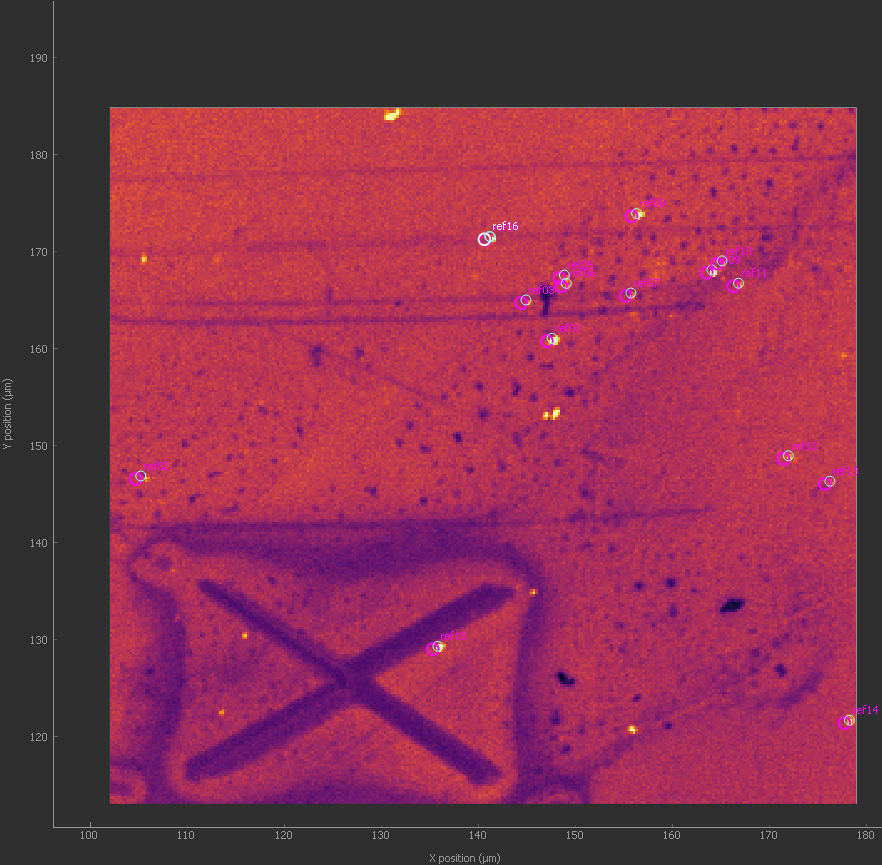
\includegraphics[width=0.7\linewidth]{Figures/pic/dc}
\caption{}
\label{fig:dc}
\end{figure}
\FloatBarrier
Once again, we exxplored the sample with the same room temperature confocal microscopy setup. With the help of spectrometer, we find a few points of interest with a emission spectrum that resembles $SiV^{-}$. 

3. Cold time-resolved PL and exitation polarisation

As has been mention in last chapter, it is suspect that the incident polarisation can affect the spectral behaviour of SiV. We added in the excitation polarisation measurement and recorded the time resolved photoluminescence spectra of 2 different excitation polarisation that are perpendicular to each other. This is achieved by putting a motor-driven half-lambda plate after the noise eater. 
Due to short time scheme from this measurement we decided to fix the input power at [?need to check], which is the lowest power that can offer most of the points of interest's a decent signal to noise ration.
\FloatBarrier
\begin{figure}[h]
\centering
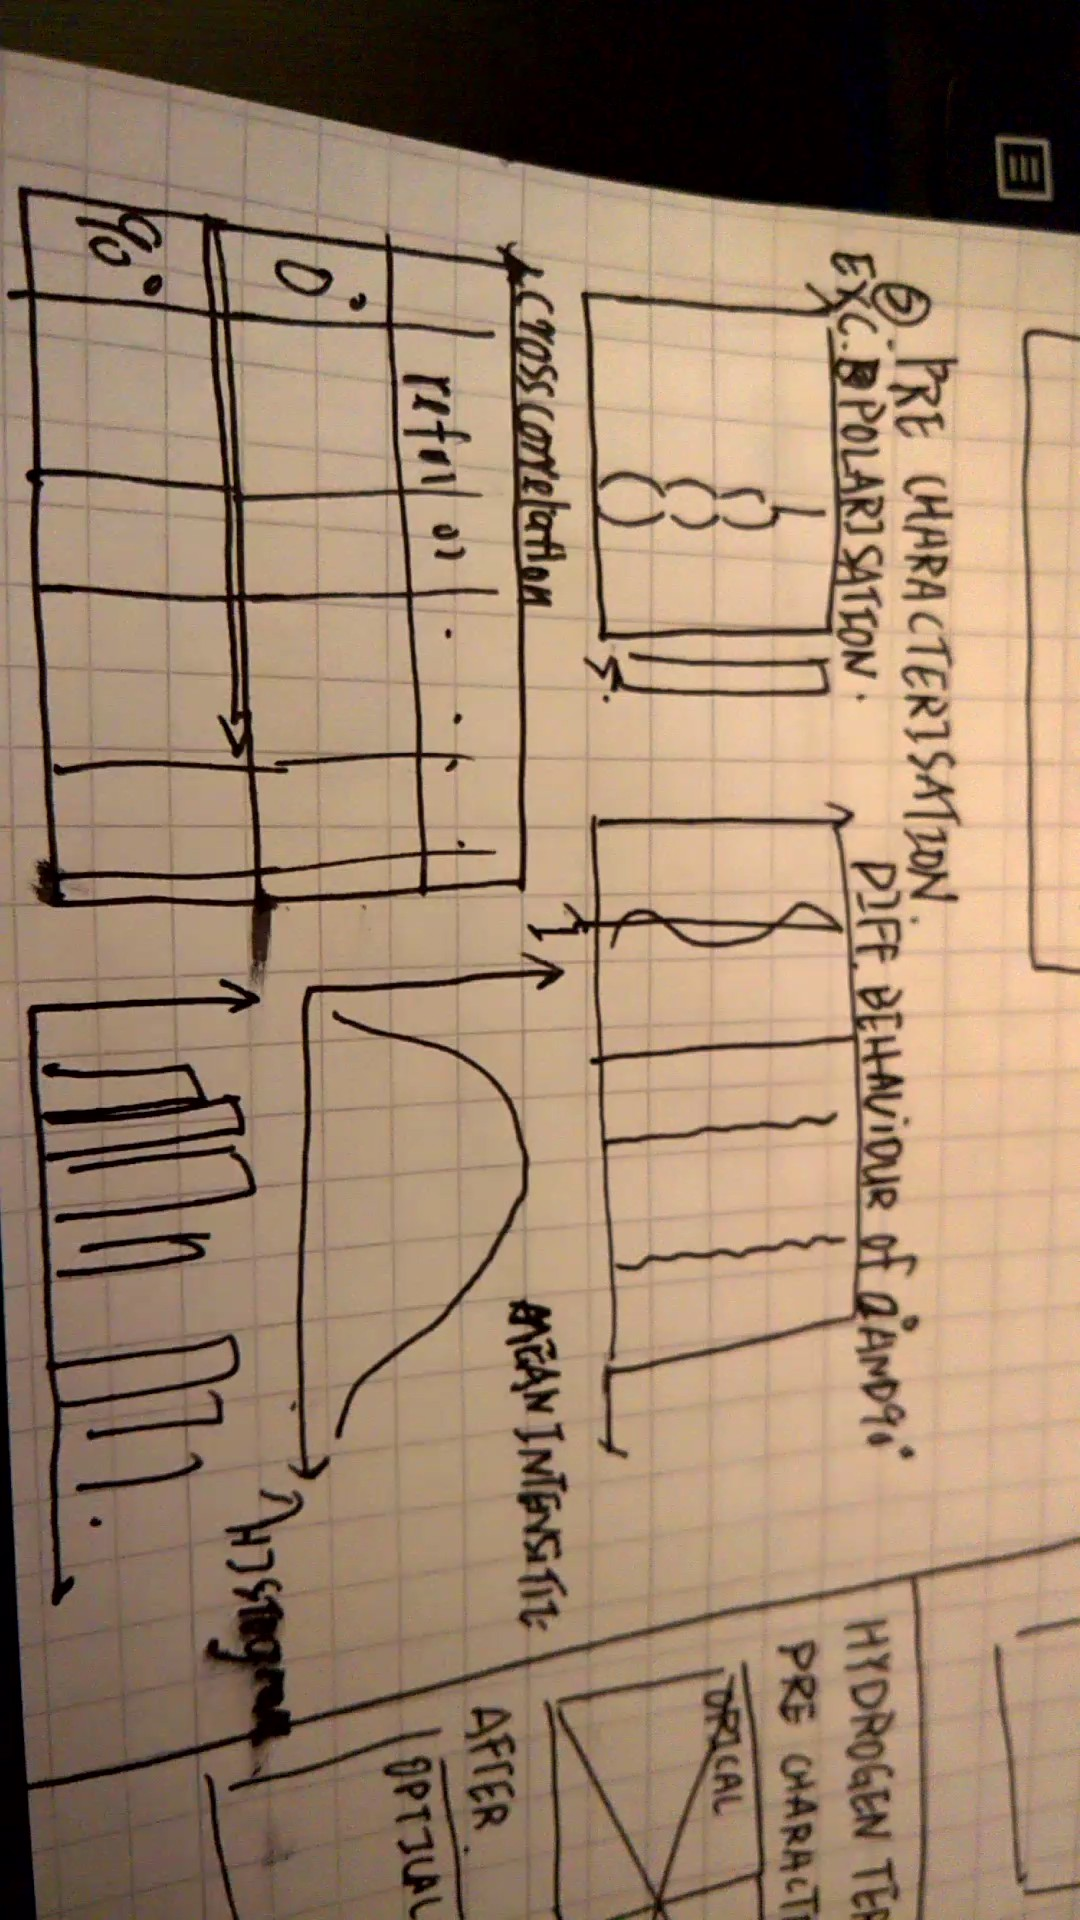
\includegraphics[width=0.7\linewidth]{Figures/pic/WP_20160921_21_04_59_Moment}
\caption{}
\label{fig:wp20160921210459moment}
\end{figure}
\FloatBarrier



\paragraph{After Oxidation} 

1. Optical Microscopy observation. 

After the Oxidation, we found the surface not as dirty as the last Oxidation. It seems a cleaner tube and flowing gas flushing do have helped suppressing the surface contamination introduced by the tube furnace.
2. Room temperature mapping
\FloatBarrier
\begin{figure}[h]
\centering
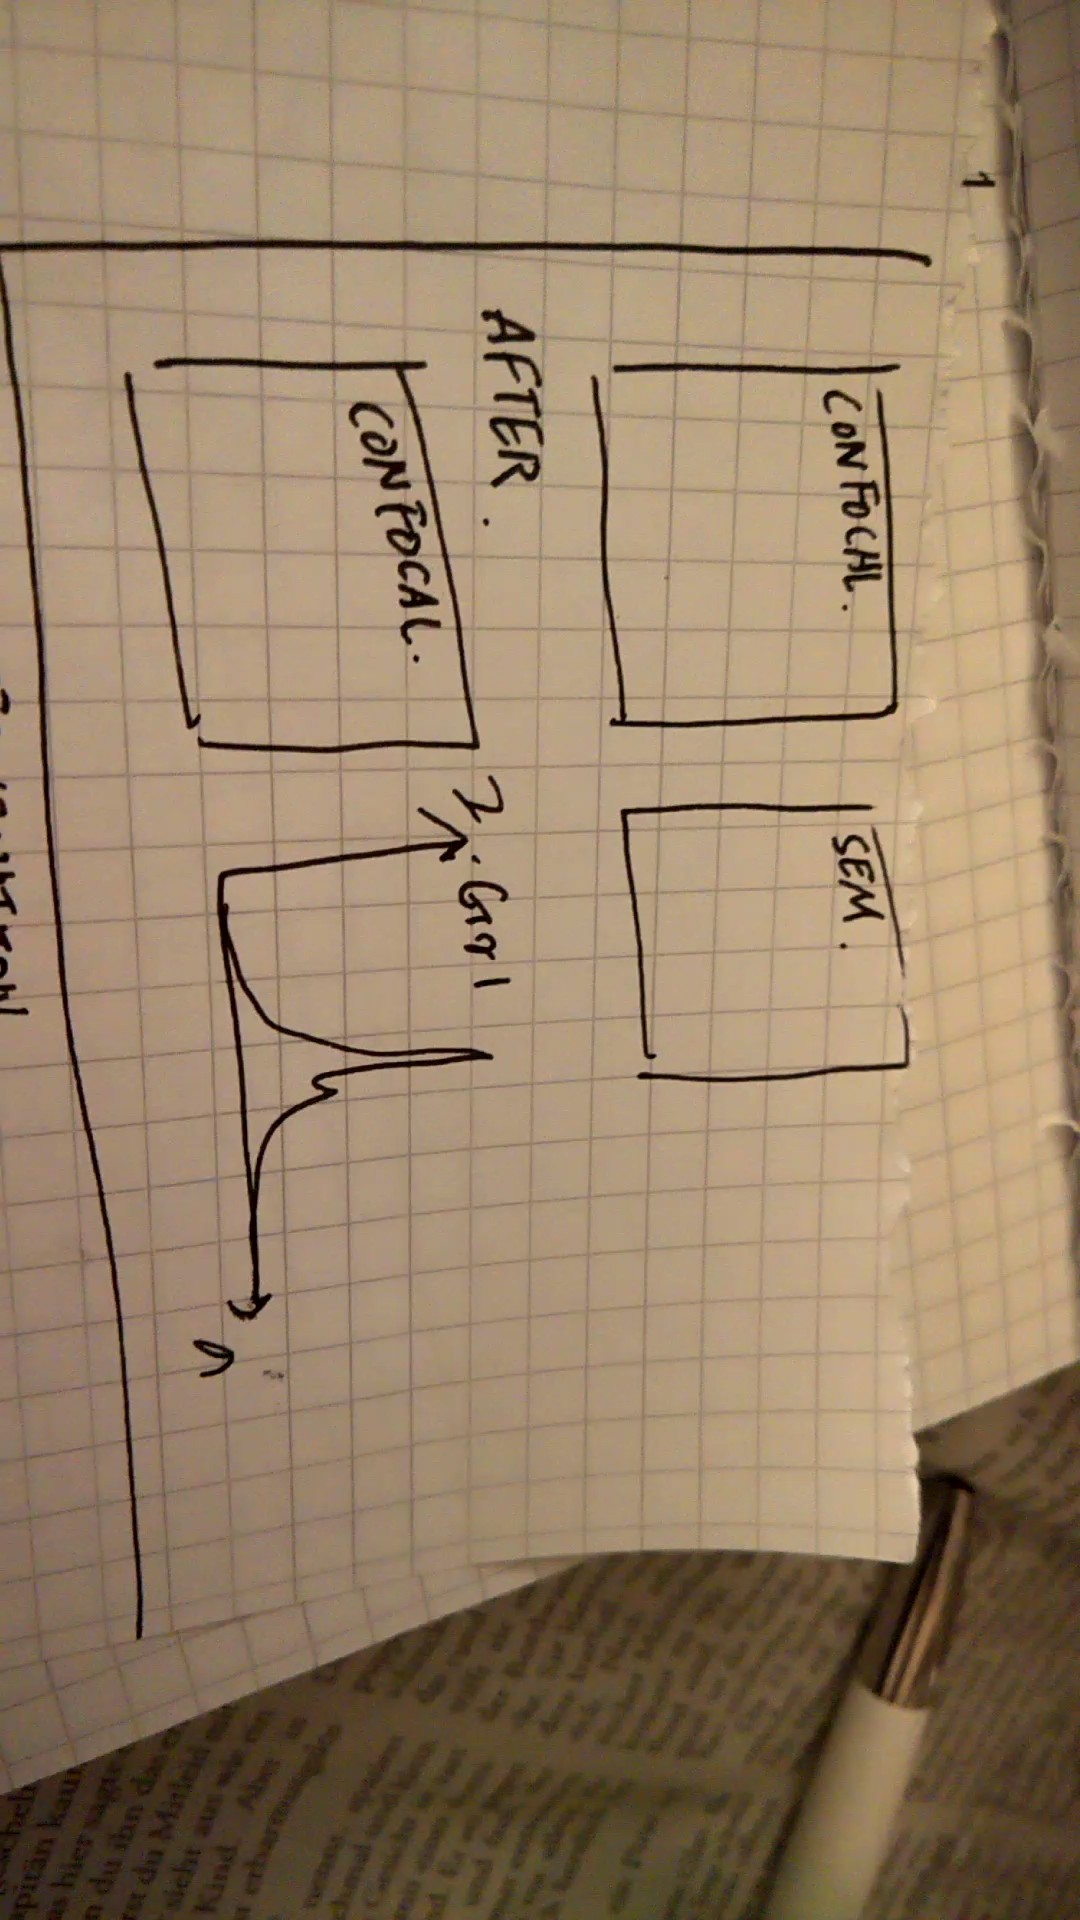
\includegraphics[width=0.7\linewidth]{Figures/pic/WP_20160921_21_05_04_Moment}
\caption{}
\label{fig:wp20160921210504moment}
\end{figure}
\FloatBarrier



\paragraph{Analysis} 
Comparasion if possible: different behaviour pre treatment between two batches
Possible reason: losing NDs due to Helium flow while cooling, GR1 getting closer to the surface due to oxidation caused size/thickness reduction.

%----------------------------------------------------------------------------------------
%	SECTION 4
%----------------------------------------------------------------------------------------

\section[H termination]{H termination}
\paragraph{Effect of H termination}

\FloatBarrier
\begin{figure}[h]
\centering
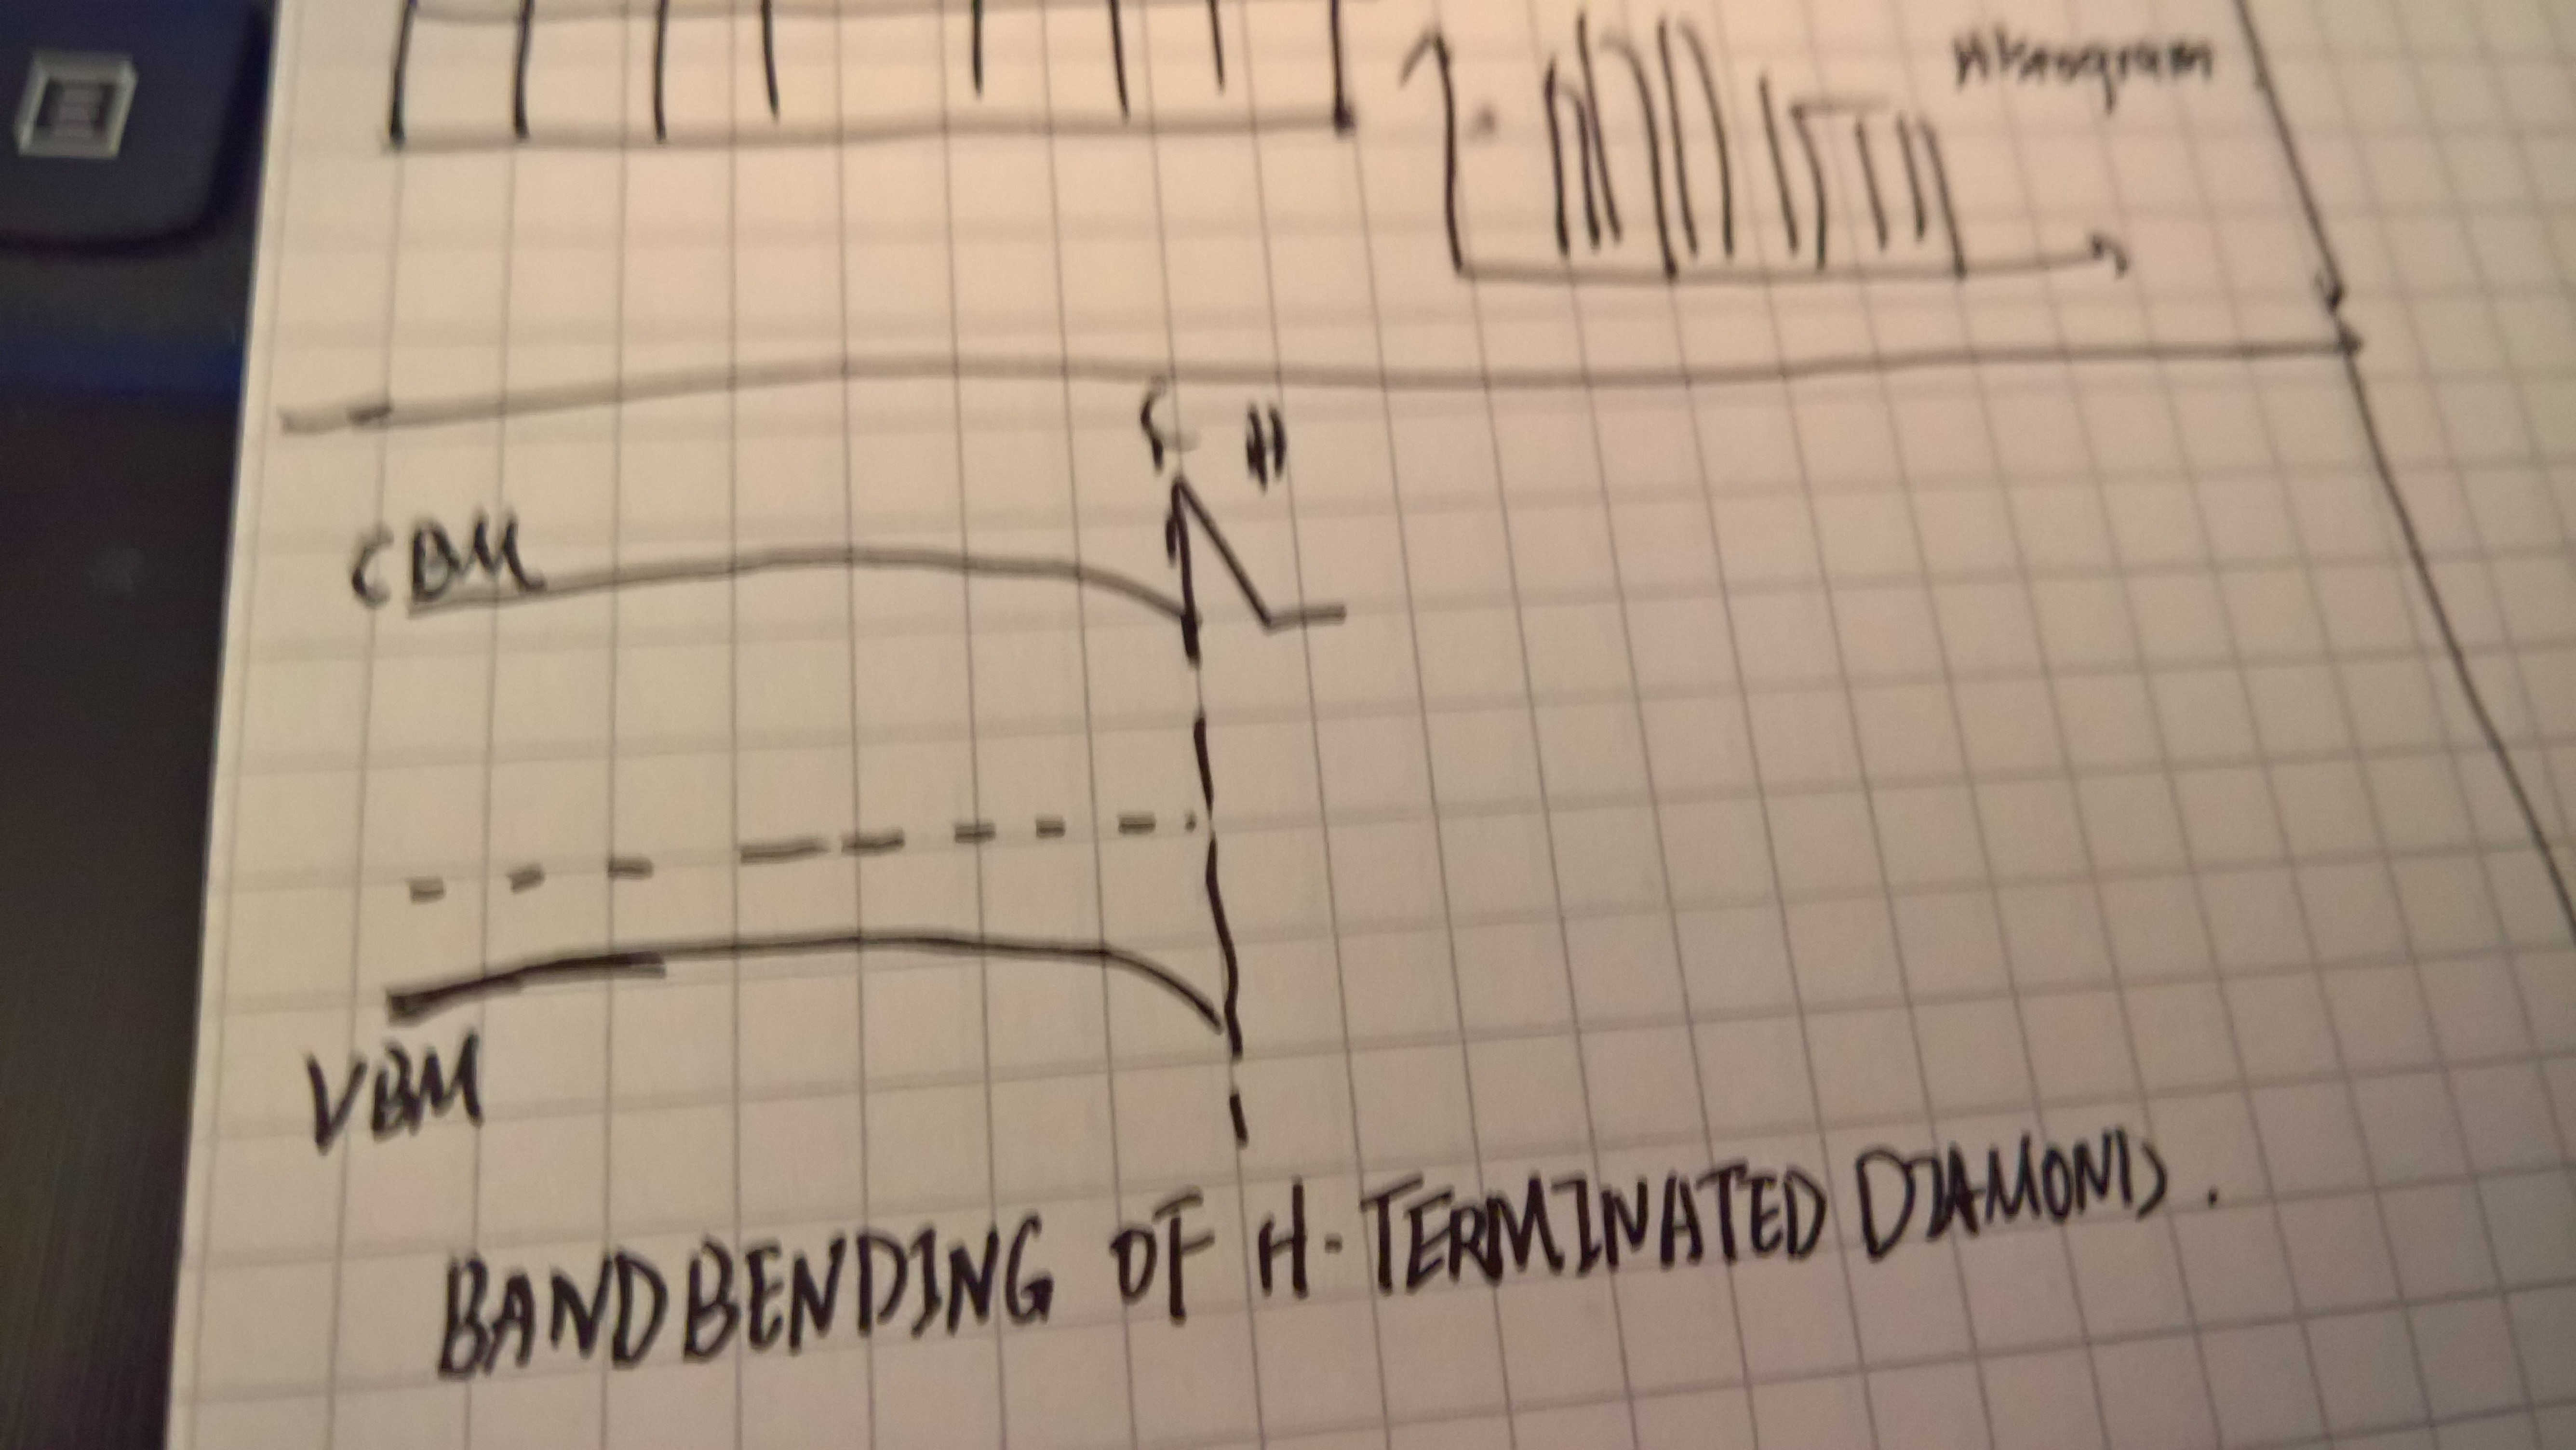
\includegraphics[width=0.7\linewidth]{Figures/pic/WP_20160921_21_05_16_Pro_LI}
\caption{}
\label{fig:wp20160921210516proli}
\end{figure}
\FloatBarrier
\paragraph{method} Plasma treatment, setup, apparatus.
ASK OSCHDI TO SEND THE PARAMETERS

\paragraph{why no pre characterisation} Conditions for Plasma treatment.
Vaccum and clean surface.
\paragraph{After H termination} Confocal image, optical image, excitation polarisation, time resolved PL with different incident polarisation.
\FloatBarrier
\begin{figure}[h]
\centering
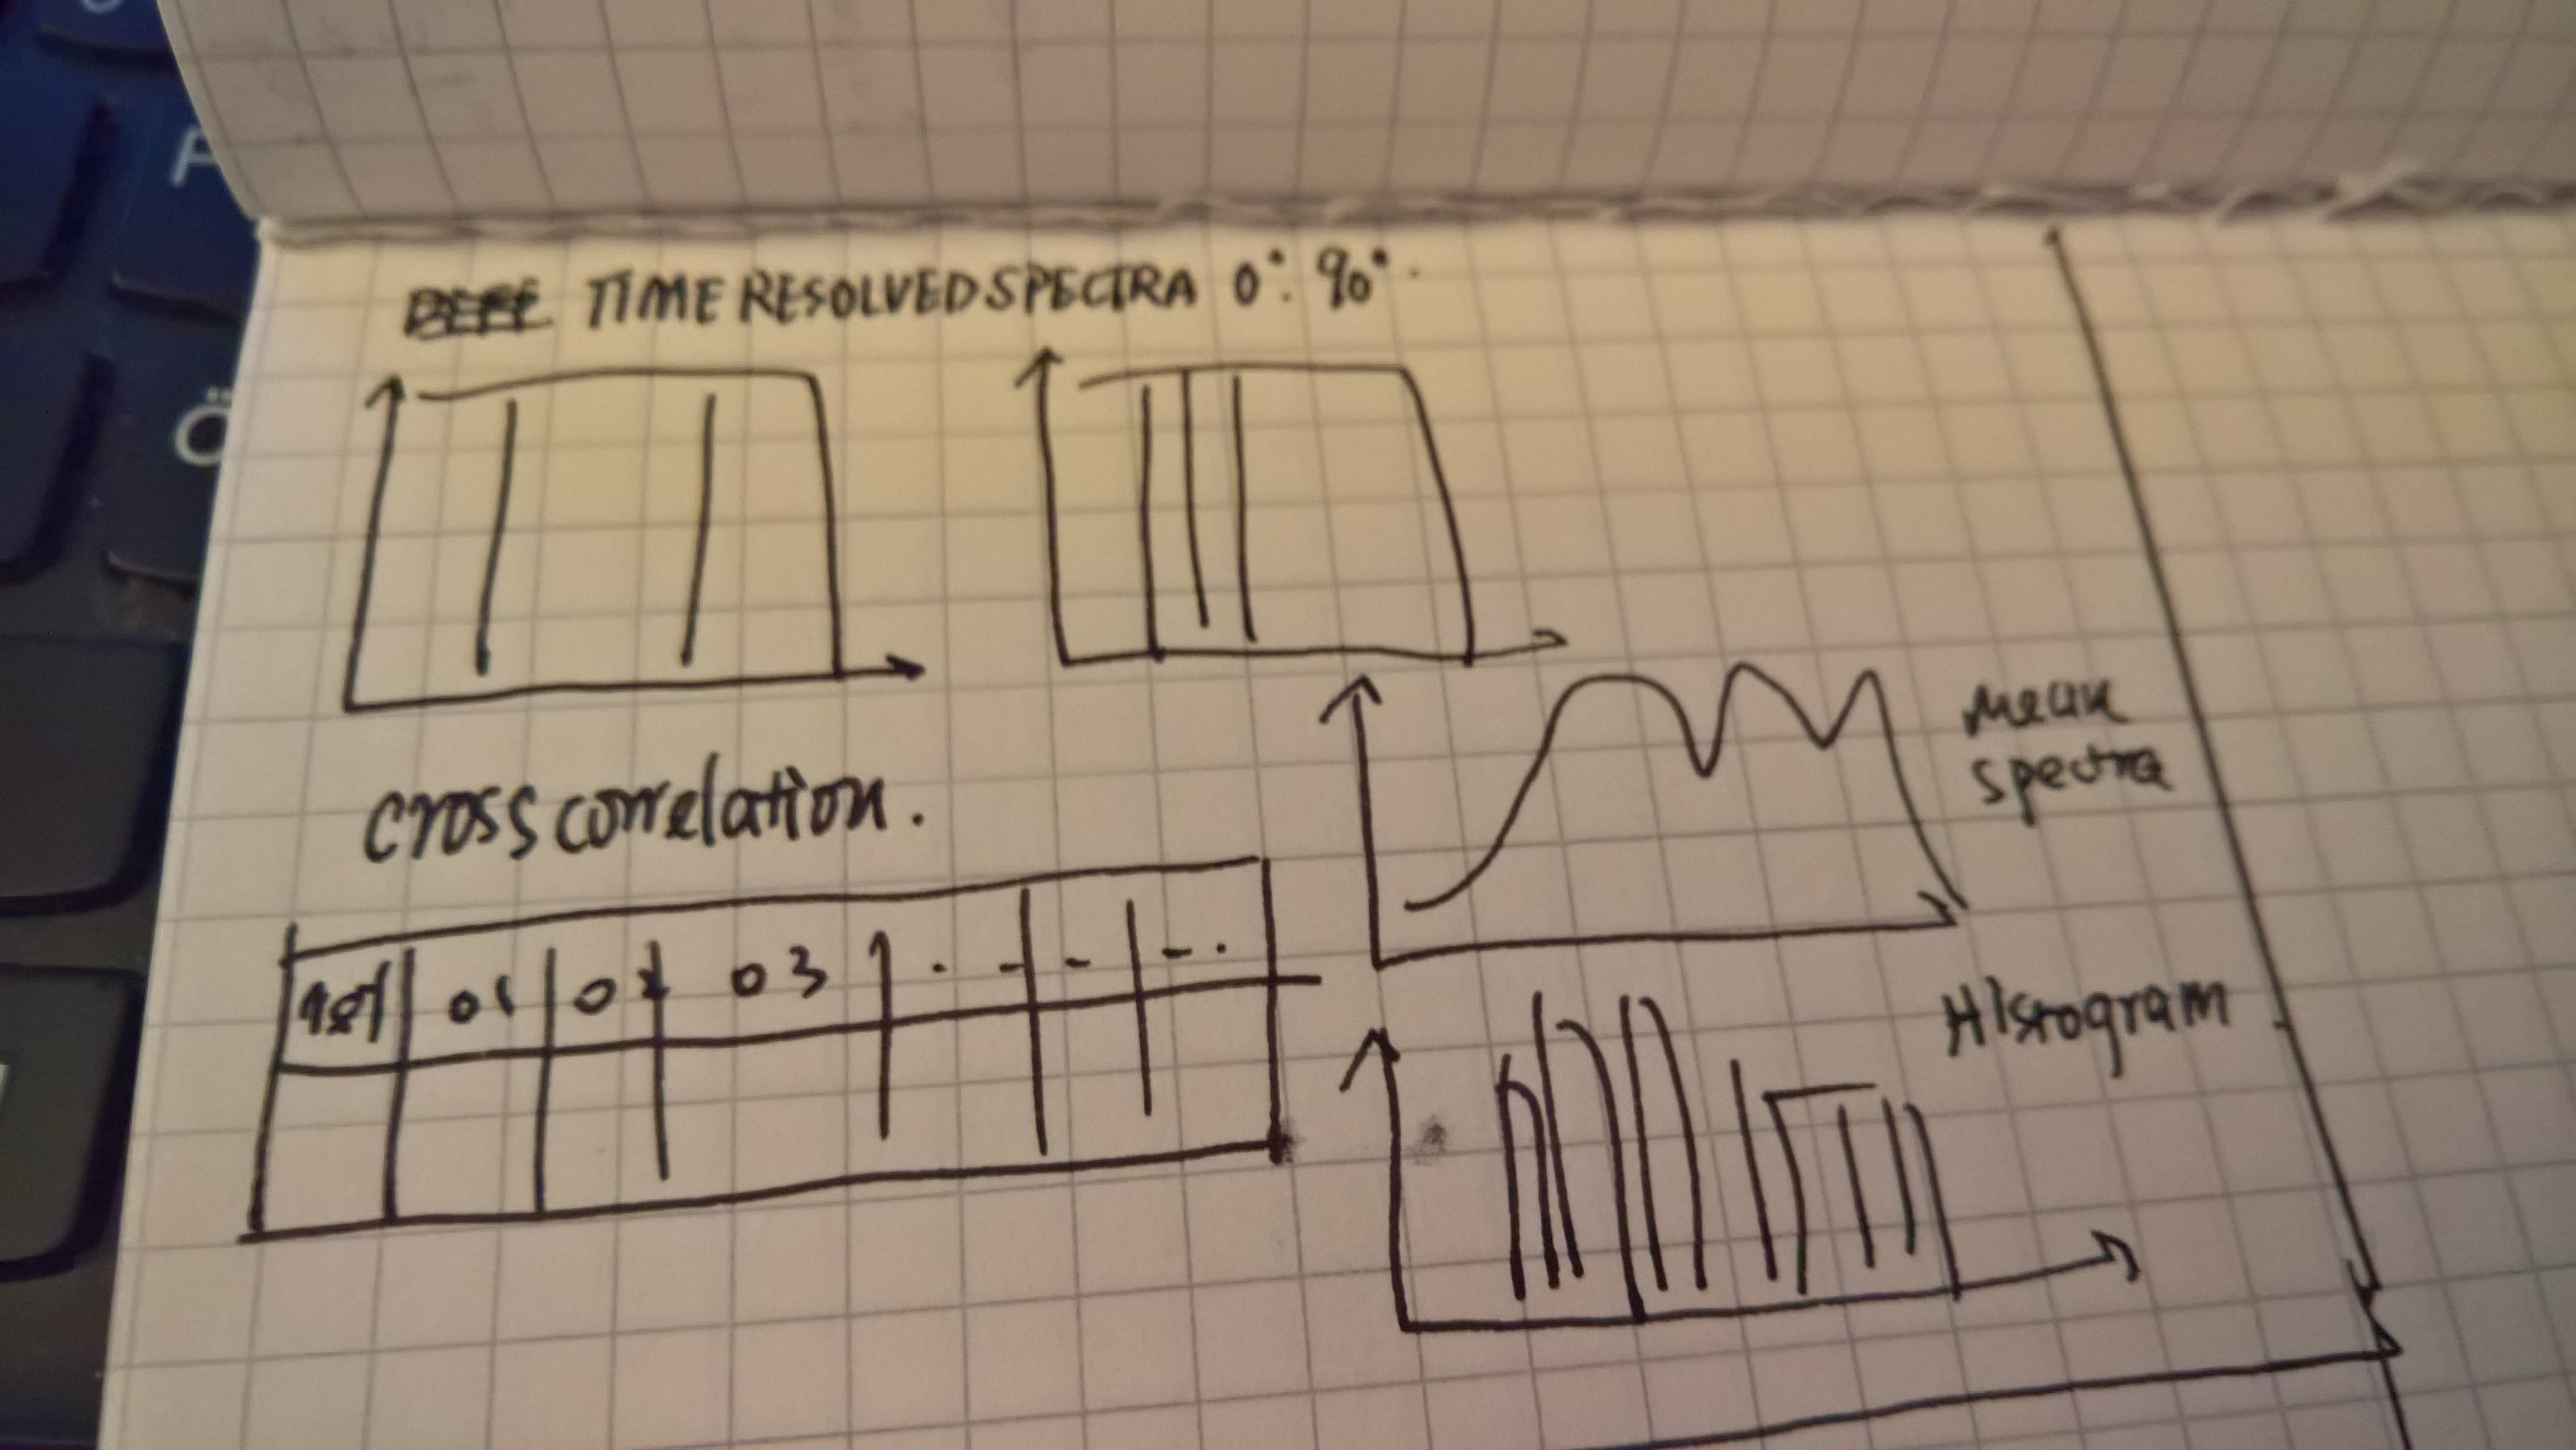
\includegraphics[width=0.7\linewidth]{Figures/pic/WP_20160921_21_05_13_Pro_LI}
\caption{}
\label{fig:wp20160921210513proli}
\end{figure}
\FloatBarrier

\paragraph{Analysis} Within the instrumental limit of spectrometer, the spectral diffusion has been significantly suppressed. Possible reason.